\chapter{Detecção utilizando métodos tradicionais} \label{chap:tradicional}

O sistema de segurança na fábrica consiste na detecção de pessoas sob a área da ponte. Esse é um problema de localização de objetos, mais especificamente, de detecção de pessoas. Tradicionalmente divide-se essa tarefa em três técnicas de visão computacional: obtenção de candidatos a objeto, obter descrição de cada candidato e então validar a amostra através de classificador. Essa solução foi baseada no trabalho de \cite{rauter}, que propõe um método de obtenção de candidatos e de extração de características. Primeiramente descreve-se aspectos técnicos da aplicação e em seguida cada uma das tarefas para a concretização da solução, por fim, pontos sobre a implementação são mencionados.

\section{Caracterização da aplicação}
Para essa aplicação, recomenda-se a utilização de imagens de profundidade, em que o valor dos pixels indicam a distância entre a câmera e o objeto em questão. Isso se deve ao fato de esse sensor fornecer uma medida independente de luminosidade e variações de cor ou textura se comparada à uma câmera RGB tradicional. Três câmeras foram compradas e avaliadas: \textit{ASUS XtionPRO}, \textit{Orbbec Astra PRO} e \textit{Stereolabs ZED}. As duas primeiras funcionam com o princípio de laser estruturado, já a última funciona baseado em visão estéreo (duas câmeras). Através de testes determinou-se que as maiores distâncias detectadas foram de 4m, 5m e 20m respectivamente. Dado que a câmera será instalada a 6m do chão, em visão superior, optou-se por utilizar a câmera \textit{ZED}.

As imagens recebidas da câmera precisam ser pré-processadas de forma a obter um mapa de distâncias, que é a imagem de profundidade. Isso é feito pela biblioteca fornecida pela \textit{Stereolabs}. Em seguida, inverte-se a imagem (subtrai-se cada pixel da distância da câmera) de maneira que cada pixel forneça a altura em relação ao chão do objeto por ele representado. Além disso pixels cujas distâncias não foram corretamente estimadas são marcados com um valor específico e o resultado é uma imagem cujos valores representam a altura dos objetos em milimetros. Essa informação é relevante pois permite obter candidatos a cabeças de maneira eficiente.

\section{Obtenção de candidatos}
\label{sec:tradicional-candidatos}
O primeiro passo consiste em obter candidatos a pessoas, como a vista é superior, candidatos a cabeças. Em uma aplicação tradicional, com câmeras RGB esse processo dividiria a imagem em pequenos blocos de tamanhos que se espera para uma cabeça, sem qualquer informação sobre o posicionamento, isto é, varrendo uma ``janela imaginária'' pela imagem.

Para aprimorar esse método, assume-se a hipótese de que cabeças serão os objetos mais altos de uma vizinhança, se destacando na cena dos demais objetos. Embora ela não seja sempre verdadeira, ao se verificar que existem máquinas altas, é um método mais eficiente de selecionar candidatos do que utilizar uma janela varrendo todo o quadro.

Aplica-se o método de máximos locais: a imagem é dividida em quadrados de áreas iguais. Para cada quadrado percorre-se os pixels e seleciona-se o maior deles, se este pixel for único no conjunto ele é considerado um ponto candidato à cabeça. Esse processo resulta num conjunto de pontos que determinam candidados à cabeças.

O tamanho dos quadrados que dividem a imagem é fundamental nessa etapa: se forem muito grandes há alta probabilidade de se perder cabeças visto que na cena existem máquinas altas. Por outro lado, se forem muito pequenos, existirão muitos candidatos e o processo se torna lento. Esse tamanho é calculado \cite{rauter} utilizando a equação 
\begin{equation}
	\label{eq:cam-proj}
	s_w = \frac{f}{d} \cdot s_r
\end{equation}
 onde $f$ é a distância focal da câmera, a $d$ a distância média entre a câmera e as pessoas e o $s_r$ o tamanho padrão de cabeças.

Em seguida, é necessário determinar um quadrado que delimite a cabeça de forma centralizada. Para obter o tamanho do quadrado, novamente utiliza-se a equação \eqref{eq:cam-proj}, porém dessa vez utilizando o valor do pixel encontrado para aquele candidato como altura. Tem-se então um quadrado de tamanho apropriado com o pixel máximo no centro, porém em poucos casos esse quadrado centraliza a cabeça.

Utiliza-se um processo de centralização baseado em \textit{mean shift}, que permite iterativamente localizar o máximo de uma função probabilidade dado uma máscara. Nesse caso, uma interpretação do procedimento é mover o quadrado mantendo suas dimensões fixas para o centróide dos pixels que estão em seu interior. Intuitivamente, percebe-se que os pixels de valor mais elevado terão maior peso, portanto, espera-se que o quadrado seja centralizado sob parte central da cabeça.

Atualiza-se o centro do retângulo
\begin{equation}
	\label{eq:mean-shift}
	m(p) = \frac{\sum_{p_i \in S(p)} I(p_i)p_i}{\sum_{p_i \in S(p)} I(p_i)}
\end{equation}
onde $I$ é a imagem e $S(p)$ é o conjunto dos pixels no quadrado de centro $p$.

\begin{figure}[h]
\centering
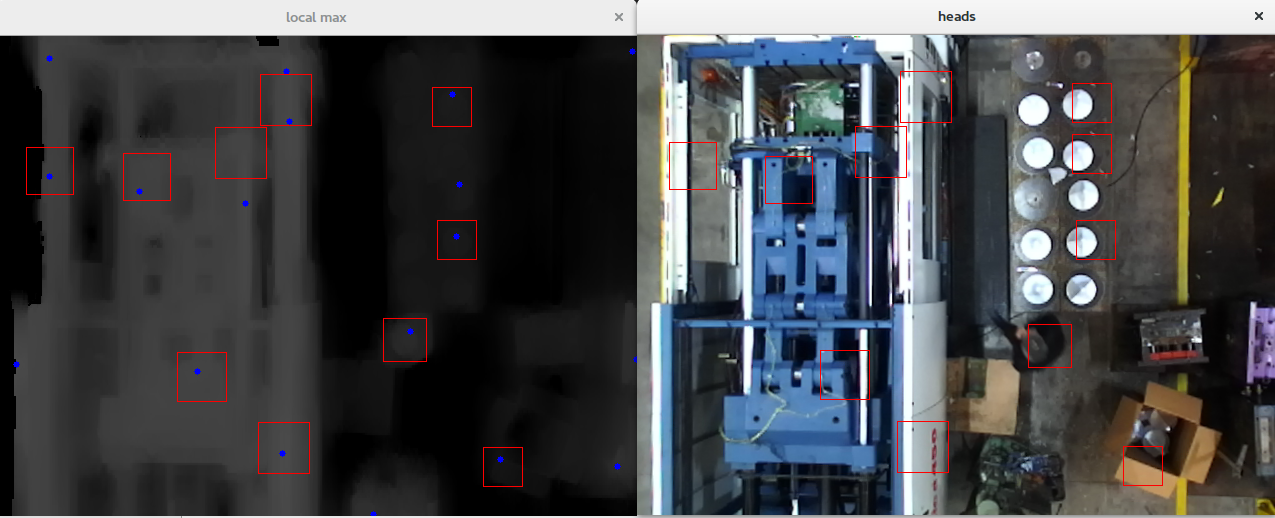
\includegraphics[width=0.8\textwidth]{tradicional/candidatos}
\caption{Pontos em azul são máximos locais e os quadrados vermelhos indicam os candidatos centralizados}
\label{fig:candidatos}
\end{figure}

Ao final dessa etapa, conta-se com uma lista de candidatos representados pelo \textit{patch} da imagem correspondente, como ilustrado na Figura \ref{fig:candidatos} pelos quadrados em vermelho.

\section{Descritores}
\label{sec:tradicional-descritores}
Tendo a lista de candidatos é necessário obter uma descrição para cada um deles. No trabalho de referência \cite{rauter} se destacam dois descritores: grades simples e grades circulares. Um terceiro descritor é proposto no presente trabalho para substituir o de grades circulares. Observa-se que para todos os descritores a característica importante de representação está nos desníveis da cabeça em relação ao resto do corpo, que se dá de maneira aproximadamente circular. Portanto, objetiva-se encontrar uma maneira de evidenciar quando e em que grau esse tipo de padrão ocorre.

O primeiro descritor, grades simples, divide o candidato em blocos, com uma quantidade ímpar em cada dimensão, como ilustrado na Figura \ref{fig:descritores}. Para esse descritor em específico, fixou-se a quantidade de blocos em 7 para cada dimensão com 49 blocos no total, pois avaliou-se que para o tamanho dos candidatos esta foi a representação mais adequada. Então calcula-se a média dos pixels em cada um dos blocos, gerando uma matriz de médias 7x7. Em seguida, subtrai-se dessa matriz o valor da média do bloco central. Por fim, gera-se um histograma da matriz resultante com número de intervalos igual a 32. Esse vetor de histograma é considerado o vetor de descrição (\textit{feature vector}), cuja soma é 49.

Já o segundo método, grades circulares, apresentado em \cite{rauter}, propõe que uma série de blocos quadrados seja disposta circularmente sobre a imagem candidata e que o mesmo procedimento do primeiro extrator seja realizado. O objetivo seria ter um descritor com maior invariância à rotação, dada a distribuição dos blocos. Porém, esse extrator é difícil de implementar devido à variação do tamanho dos candidatos.

Para facilitar a implementação, propomos, então, um descritor de anéis concêntricos. A ideia é similar às grades circulares, porém ao invés de se dispor blocos de maneira circular, utilizam-se coroas que partem desde o centro da imagem até as bordas. Primeiramente divide-se a imagem em $n$ coroas circulares cujo centro coincide com o da imagem e cuja diferença entre os raios é constante, como visto na Figura \ref{fig:descritores}. Então gera-se um vetor $v \in \RR^n$ em que cada elemento corresponde à média dos pixels pertencentes à $n$-ésima coroa, desconsiderando os pixels inválidos. Em seguida subtrai-se desse vetor o valor da média da primeira coroa, cujo raio menor é 0 correspondendo então à um círculo. Por fim a descrição do candidato corresponde à diferenciação discreta (diferenças entre as componentes adjacentes) desse vetor, para evidenciar ainda mais as diferenças entre as alturas médias das coroas. Note que o vetor de descrição tem dimensão $d=n-1$. Para esse descritor diferentes valores de $n$ foram avaliados para identificar a melhor divisão, conforme descrito no Capítulo \ref{chap-resultados}.

Após obter a descrição de cada candidato é possível classificá-los de maneira a validar que são cabeças de fato.

\begin{figure}[h]
\centering
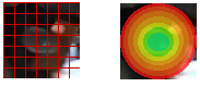
\includegraphics[width=0.8\textwidth]{tradicional/descritores}
\caption{Ilustração dos descritores: grades simples e anéis concêntricos.}
\label{fig:descritores}
\end{figure}

\section{Classificação}
\label{sec:classificacao:svm}
%Referência SVM http://www.cs.columbia.edu/~kathy/cs4701/documents/jason_svm_tutorial.pdf

Utiliza-se um classificador binário SVM (\textit{Support Vector Machine}). Seja o dataset o conjunto $(x_i, y_i)$ para $i=1 \dots N$ com $x_i \in \RR^d$ sendo o vetor de descrição do candidato $i$ e $y_i \in \{-1, 1\}$ sendo a classe correspondente, não-cabeça ou cabeça, respectivamente. Deseja-se encontrar um classificador $f(x)$ tal que 
\begin{equation*}
\label{eq:svm-decision}
	\begin{cases}
		f(x_i)>0,& \text{se } y_i=1 \\
		f(x_i)<0,& \text{se } y_i=-1 \\
	\end{cases}
\end{equation*}
 ou seja, $y_i f(x_i) > 0$ para uma classificação correta. 

A função de decisão do SVM pode ser descrita como $f(x)=w^T x+ b$ onde $w \in \RR^d$ é o vetor de pesos, que fornece a inclinação do hiperplano e $b \in \RR$ um deslocamento do hiperplano em relação à origem. Define-se ainda a margem como a menor distância entre o hiperplano de separação e qualquer amostra, dada por $\frac{2}{\|w\|}$ onde
\begin{equation}
\|w\| = \sqrt{w_1^2 + \dots + w_n^2}.
\end{equation}

O aprendizado consiste em encontrar $w$ e $b$ que maximizem a a margem sujeitos à $y_i(w^T x_i+b) \geq 1$. Esse é um problema de otimização convexa, em que qualquer mínimo local é também global. Assim, minimiza-se a função custo \cite{bishop2007}
\begin{equation}
	\label{eq:svm-cost}
	\min P(w,b) = \frac{1}{2}\|w\|^2 + C\sum_i H_1(y_i f(x_i)).
\end{equation}
onde a função
\begin{equation*}
H_1(z)=\max(0,1-z)
\end{equation*}
é utilizada para dar um peso negativo quanto maior for o erro do classificador (quando o argumento é negativo).

O primeiro termo da equação \eqref{eq:svm-cost} está associado à maximização da margem e o segundo à minimização dos erros de treinamento, quando uma amostra é classificada erroneamente. O parâmetro $C$ controla quanto se penaliza os erros de classificação diante da maximização da margem, visto existir uma relação ideal entre eles.

O dataset é considerado linearmente separável se for possível encontrar uma reta ou hiperplano que separe todas as amostras corretamente. Entretanto nem sempre que for linearmente separável a classificação sem erros é o ideal. Por exemplo, o dataset apresentado Figura \ref{fig:svm-margin} mostra que optar pela separação ótima gera perda de generalização. Fica evidente que nesse caso deveria-se priorizar uma margem maior em detrimento de alguns possíveis erros de classificação, o que pode ser feito diminuindo o valor de $C$.

\begin{figure}
\centering
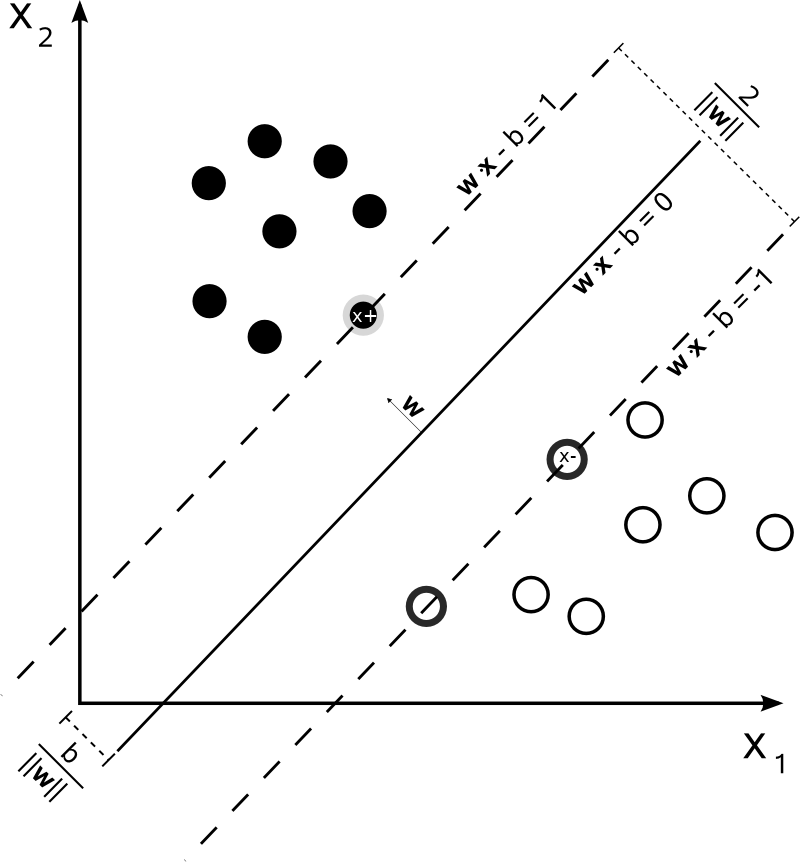
\includegraphics[width=0.3\textwidth]{svm/svm-margin}
\caption{Exemplos de dataset em que separação perfeita não é ideal}
\label{fig:svm-margin}
\end{figure}

O modelo de SVM apresentado até aqui é conhecido como linear. Mesmo com o método de penalização de erros de classificação, datasets complexos podem não ter um desempenho satisfatório. Dessa maneira, é introduzido um modelo não linear para o classificador: transforma-se as amostras $x_i$ em um novo espaço obtendo amostras $\Phi(x_i)$ que são, no caso ideal, linearmente separáveis, como mostrado na Figura \ref{fig:svm-kernel}.

\begin{figure}
\centering
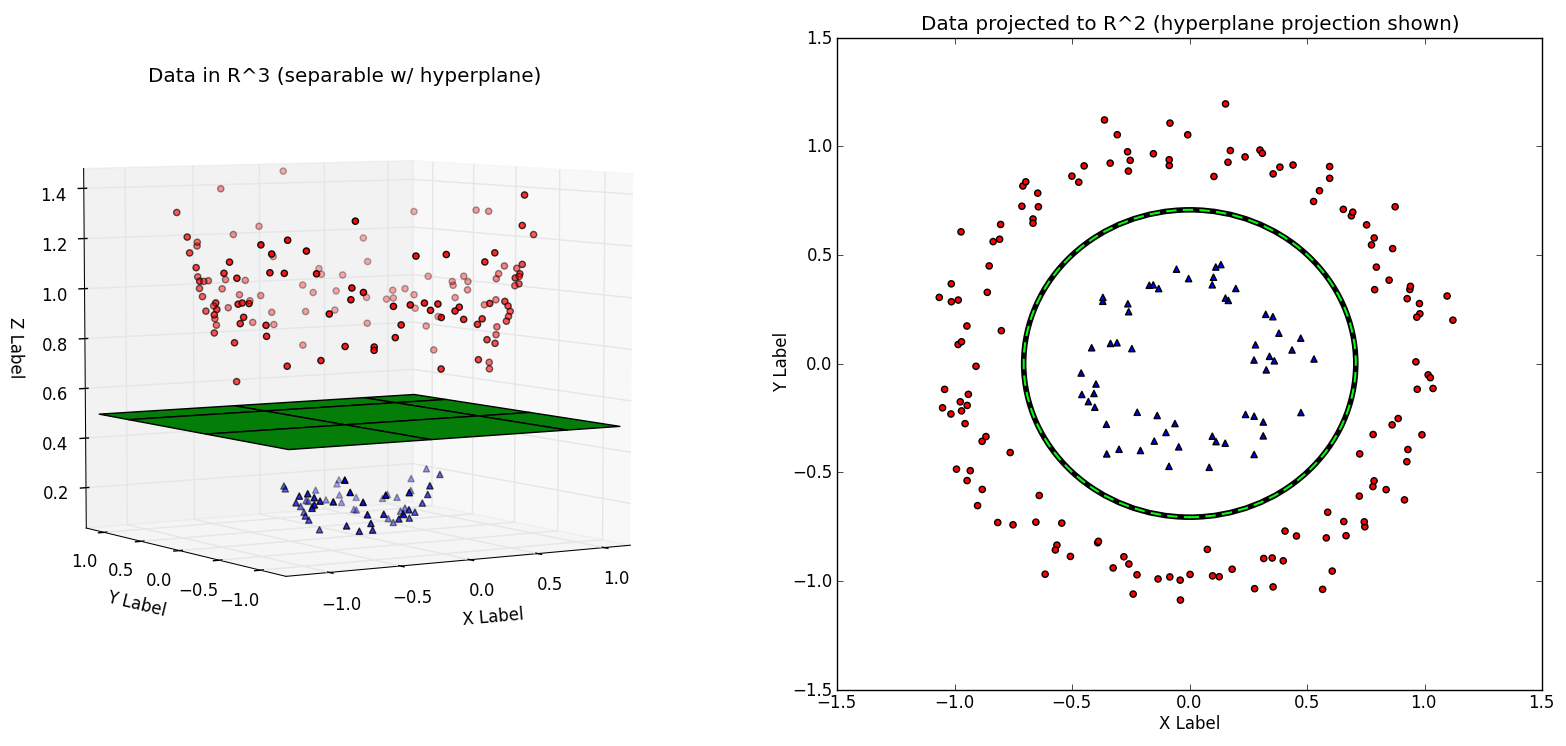
\includegraphics[width=0.8\textwidth]{svm/svm-kernel}
\caption{Exemplo de mapeamento para obter um classes linearmente separáveis. Espaço transformado e original, respectivamente.}
\label{fig:svm-kernel}
\end{figure}

Formalmente \cite{bishop2007} tem-se a função decisão modificada como
\begin{equation*}
f(x)=w^T \Phi(x) +b.
\end{equation*}
Na prática, entretanto, não se calcula as coordenadas da amostra transformada no novo espaço. Ao invés disso utiliza-se o chamado \textit{kernel trick} \cite{bishop2007} em que o produto interno entre duas amostras transformadas é obtido diretamente através da avaliação da função $\Phi(x)$ sob as amostras originais.

Segue do teorema da representação de Kimeldorf e Wahba \cite{kimeldorf1970correspondence} que
\begin{equation}
	\label{eq:teo-kimeldorf}
	w=\sum_{i=1}^m \alpha_i \Phi(x_i)
\end{equation}
para alguma variável $\alpha$. Portanto, ao invés de minimizar $w$ diretamente, podemos minimizar $\alpha$ e a função decisão se torna
\begin{equation}
	\label{eq:svm-decision-func}
	f(x)=\sum_{i=1}^m \alpha_i \Phi(x_i) \Phi(x) +b.
\end{equation}

Chamamos $K(x_i, x) = \Phi(x_i) \cdot \Phi(x)$ de \textit{kernel} ou função núcleo. Um exemplo bastante utilizado é a \textit{Radial Basis Function} (RBF), também conhecida como núcleo gaussiano, dada por
\begin{equation}
	\label{eq:svm-kernel-func}
	K(x,x_i) = \exp\left(-\frac{\|x-x_i\|^2}{2\sigma^2}\right).
\end{equation}
Nota-se que quando $\|x-x_i\|$ é muito maior que $\sigma$ a função retorna um valor que tende a zero, o que demonstra que a amostra em questão tem pouca importância para o hiperplano de decisão. Assim, quanto menor o valor de $\sigma$, mais local tende a ser o classificador, o que faz com que o desempenho no conjunto de treinamento seja excelente. Porém, ao mesmo tempo proporciona menor generalização do modelo, o que significa que esse desempenho não se replica no conjunto de teste.

\section{Variação para saída probabilística}
\label{sec:svm-probabilistic}
A formulação tradicional do SVM possui saída categórica, isto é, a classe à qual a amostra pertence. Entretanto, para uma classificação binária, é possível adicionar um componente que permite estimar uma saída probabilística, isto é, a probabilidade da amostra ser positiva.

A função de decisão \eqref{eq:svm-decision} é proporcional à distância (com sinal) da amostra até o hiperplano de separação. Redimensionando essa medida através da função de Platt \cite{svmProbabilisticOutput} é possível obter a probabilidade da amostra pertencer à determinada classe $P(y_i=1 | x_i)$. A função de Platt é simplesmente uma regressão logística, cujos parâmetros são encontrados por otimização após o treino do SVM tradicional. Permitindo, então, obter uma saída probabilística de um classificador SVM.

Essa formulação é interessante pois dá flexibilidade do rigor da classificação através da escolha do limiar de probabilidade a partir do qual uma amostra é considerada positiva após o modelo ter sido treinado.

\section{Implementação}
Para os algoritmos de processamento de imagens e extração de características, fez-se uso da biblioteca \textit{OpenCV} que implementa grande quantidade de operações básicas em imagens e fornece um ambiente rico de trabalho para criar novas funcionalidades.

No que se refere a aprendizado de máquina, utilizou-se a biblioteca \textit{Scikit-learn} \cite{scikit-learn} que implementa o algoritmo de treinamento SVM. Além de fornecer as amostras, no caso, a descrição dos candidatos, é necessário configurar os parâmetros $C$, para penalidade dos erros de treinamento e o parâmetro $\sigma$ do \textit{kernel RBF}. 

A abordagem utilizada foi o método de treinamento automático fornecido pela biblioteca: indica-se um conjunto de elementos para cada um dos parâmetros e todas as combinações de parâmetros são testadas utilizando um processo de validação cruzada. Basicamente divide-se o conjunto de treinamento em 5 conjuntos dos quais quatro são utilizados para treinamento e um para validação. Ao final do procedimento as estatísticas de cada tentativa é exibida e a que tiver melhor desempenho, segundo métrica estabelecida, é escolhida. Tendo obtido esses parâmetros um novo processo de treinamento é efetuado, agora utilizando todo o conjunto de treinamento, sem validação.

Nota-se ainda que é possível utilizar de todos os núcleos do processador com essa biblioteca, o que traz um impacto bastante positivo na performance temporal do algoritmo.

Tendo treinado o modelo é possível obter o resultado da classificação para cada candidato e remover os que não forem reconhecidos como cabeças. O resultado final do processo é um vetor de quadrados contendo todas as cabeças encontradas no quadro.
